
\section{Monday for MAT3006}\index{Monday_lecture}

\paragraph{Reviewing}
\begin{itemize}
\item
The collection of all Lebesgue measurable subsets, denoted by $\mathcal{M}$,
is a $\sigma$-algebra
\item
Borel $\sigma$-algebra: the smallest $\sigma$-algebra containing all the intervals of $\mathbb{R}$:
\begin{proof}[Well-definedness]
Let $\mathcal{S}=\{\text{all $\sigma$-algebras containing all the inervals of $\mathbb{R}$}\}$.
For example, $\mathbb{P}(R)\in\mathcal{S}$.
Note that $\forall f_i\in\mathcal{S}$, $\cap_{i\in I}\mathcal{A}_i\in\mathcal{S}$.

Then define 
$\mathcal{B}=\cap_{\mathcal{A}\in\mathcal{S}}\mathcal{A}$, 
which is the smallest $\sigma$-algebra containing all intervals.
\end{proof}

Furthermore, $\mathcal{M}\in\mathcal{S}$. Therefore, $\mathcal{B}\subseteq\mathcal{M}$ but they are not equal.
(Check Royden's note on blackboard, there exists a counter-example $A$ such that $A\in\mathcal{M}$ but $A\notin\mathcal{B}$.)

\item
The set $\mathcal{M}$ has a good property: 
If $N\in\mathcal{M}$ is null, 
then all $E\subseteq N$ are null sets, 
and therefore $E\in\mathcal{M}$.

The probelm is that it is not necessary the case that $N'\in\mathcal{B}$ implies $m\mid_{\mathcal{B}}(N')=0$, i.e., $E'\in\mathcal{B},\forall E'\subseteq N'$ does not necessarily hold.

(check back to the Roydon's counter-example)
\item
Therefore, we need the \emph{completion process} of $\mathcal{B}$ to get $\mathcal{M}$.
\end{itemize}

\subsection{Measurable Functions}
\paragraph{Motivation}
The Riemann integration divides the function into a grid of 1 (unit) squares, and then measure the altitude of the function at the center of each square.
Therefore, the total ``volume'' of this function is 1 times the sum of the altitudes.

However, the Lebesgue integraion aims to study the vertical length of the function, and the total volumn of this function is 1 times the sum of the vertical lengths.
\begin{figure}
\centering
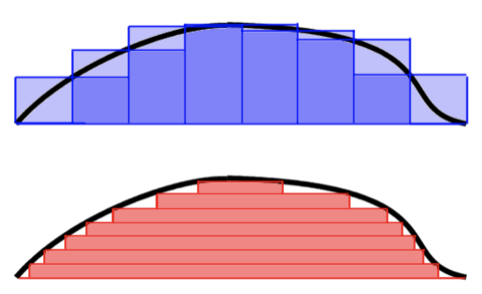
\includegraphics[width=0.45\textwidth]{week9/p_1}
\caption{Riemann Integration (in blue) and Lebesgue Integration (in red)}
\end{figure}
Riemann integration


\begin{definition}[Measurable]
Let $f:(\mathbb{R},\mu,m)\to\mathbb{R}$ be a function.
We say $f$ is \emph{(Lebesgue) measurable} if $f^{-1}(I)\in\mathcal{M}$ for all intervals $I\subseteq\mathbb{R}$.
\end{definition}

\begin{proposition}
If $f:\mathbb{R}\to\mathbb{R}$ is continuous, 
then $f$ is measurable.
\end{proposition}
The trick during the proof is to check only intervals of the form $(a,\infty)$ instead of checking all intervals in $\mathbb{R}$.
\begin{proof}
\begin{enumerate}
\item
By continuity of $f$, $f^{-1}((a,\infty))$ is open in $\mathbb{R}$.
\begin{itemize}
\item
Note that any open set $U$ can be expressed as a countable union of open intervals:
for given $q\in\mathbb{Q}$, define the set
\[
I_q=\bigcup_{\text{$I$ is an open interval, $q\in I\subseteq U$}}I,
\]
which is a union of non-disjoint open intervals, hence an open interval as well. We claim that $U\subseteq\cup_{q\in\mathbb{Q}\cap U} I_q$:

Consider any $x\in U$. When $x\in\mathbb{Q}$, the result is clear; otherwise there exists an open interval $(x-\varepsilon,x+\varepsilon)\subseteq U$. By the denseness of $\mathbb{Q}$, there exists $q\in\mathbb{Q}$ such that $q\in(x-\varepsilon,x+\varepsilon)$. By definition of $I_q$, $(x-\varepsilon,x+\varepsilon)\in I_q$. Therefore, $x\in I_q$.

The proof for this statement is complete.
\end{itemize}
Therefore, 
\[
f^{-1}((a,\infty))=\cup_{i=1}^\infty U_i\in\mathcal{M}
\]
since each open interval $U_i\in\mathcal{M}$
\item
For other types of intervals,
e.g., 
$[a,\infty)$, consider
\[
\bigcap_{n=1}^\infty(a-\frac{1}{n},\infty)=[a,\infty),
\]
which follows that 
\[
f^{-1}([a,\infty)) = f^{-1}(\bigcap_{n=1}^\infty(a-\frac{1}{n},\infty))
=
\cap_{n=1}^\infty f^{-1}((a-\frac{1}{n},\infty))\in\mathcal{M}
\]
The proof for other types of intervals needs similar reformulations of them:
\begin{align*}
f^{-1}((-\infty,a))&=f^{-1}(\mathbb{R}\setminus[a,\infty))
=
\mathbb{R}\setminus f^{-1}([a,\infty))\in\mathcal{M}\\
f^{-1}((b,a))&=f^{-1}((-\infty,a))\cap f^{-1}((b,\infty))\in\mathcal{M}
\end{align*}
\end{enumerate}

\end{proof}
\begin{remark}
\begin{enumerate}
\item
From the proof above we also find:
the function $f$ is measurable if and only if $f^{-1}((a,\infty))\in\mathcal{M}$, for $\forall a\in\mathbb{R}$.
\item
Homework question:
the function $f$ is measurable if and only if $f^{-1}(B)\in\mathcal{M}$ for $\forall B\in\mathcal{B}$.
\end{enumerate}
\end{remark}

\begin{proposition}
\begin{enumerate}
\item
Constant functions, 
and monotone functions are measurable
\item
If $A\subseteq\mathbb{R}$ is measurable, 
then the characterstic function
\[
\mathcal{X}_A(x):=\left\{
\begin{aligned}
1,&\quad\text{if $x\in A$}\\
0,&\quad\text{if $x\notin A$}
\end{aligned}
\right.
\]
is measurable.
\item
If $f$ is measurable, $h$ is continuous, then $h\circ f$ is continuous.
\item
If $f,g$ are measurable, then so is 
\[
\begin{array}{llll}
f+g,&fg,&\max/\min(f,g),&|f|
\end{array}
\]
\end{enumerate}
\end{proposition}
\begin{proof}
\begin{itemize}
\item
(1) and (2) are easy to show.
\item
The proof for (3) is simply by applying the formula
\[
(h\circ f)^{-1}((a,\infty)) = f^{-1}(h^{-1}(a,\infty)),
\]
\item
The proof for the measurability of $f+g$ is by definition:
\begin{align*}
(f+g)^{-1}(a,\infty) &= \{x\mid f+g\in(a,\infty)\}\\
&=
\cup_{q\in\mathbb{Z}}(\{x\mid f\in (q,\infty)\}\cap\{x\mid g\in(a-q,\infty)\})\\
&=\cup_{q\in\mathbb{Z}}(f^{-1}(q,\infty)\cap f^{-1}(a-q,\infty))\in\mathcal{M}
\end{align*}
The measurability of $fg,|f|,\max/\min(f,g)$ are by the equalities
\begin{align*}
fg&=\frac{1}{4}[(f+g)^2+(f-g)^2]\\
|f|&=h\circ f\quad h(x)=|x|\\
\max/\min(f,g)&=\frac{1}{2}(f+g\pm|f-g|)
\end{align*}
\end{itemize}
\end{proof}


\begin{remark}
If both $f,g$ are measurable, then $g\circ f$ is not necessarily measurable.
\end{remark}


\begin{definition}[Almost Everywhere]
Let $f,g:(\mathbb{R},\mu,m)\to\mathbb{R}$.
We say $f=g$ almost everywhere (a.e.)
if $E:=\{x\mid f(x)\ne g(x)\}$ is a null set.

More generally, we say $f(x) $satisfies a condition on $(R,\mu,m)$ a.e. if the set
\[
\{x\mid\text{$f(x)$ does not satisfy the condition}\}\ \text{is a null set}.
\]
\end{definition}
For example, the characteristic function $\mathcal{X}_{\mathbb{Q}}(x)$ is equal to zero function a.e.

The measurability ignores the null set.
\begin{proposition}\label{pro:9:3}
Suppose that $f$ is measurable, and $g=f$ a.e., then $g$ is measurable.
\end{proposition}
\begin{proof}
Note that 
\[
g^{-1}((a,\infty)) = \{x\mid g(x)\in(a,\infty), g(x)=f(x)\}\cup
\{x\mid g(x)\in(a,\infty), g(x)\ne f(x)\}
\]
where $\{x\mid g(x)\in(a,\infty), g(x)\ne f(x)\}\subseteq E$, i.e., belongs to $\mathcal{M}$;
and
\[
 \{x\mid g(x)\in(a,\infty), g(x)=f(x)\} = f^{-1}((a,\infty))\cap E^c\in\mathcal{M}.
\]

\end{proof}

\begin{remark}
During the proof, we have used the fact that $N\subseteq E$ is measurable for all null set $E$.
\end{remark}

\begin{definition}[Measurable on extended real line]
A function $f:\mathbb{R}\to[-\infty,\infty]$ is measurable if 
$f^{-1}(I)\in\mathcal{M}$ for all intervals $I\in[-\infty,\infty]$.

Following the similar idea of previous examples, it suffices to show that
\[
f^{-1}((a,\infty])\in\mathcal{M},\quad
\forall a\in\mathbb{R}.
\]
Or equivalently,
\[
f^{-1}(B)\in\mathcal{M},\forall B\in\mathcal{B},\text{ and }f^{-1}(\{-\infty\}),f^{-1}(\{\infty\})\in\mathcal{M}.
\]
\end{definition}
Example:
\[
f(x)=\left\{
\begin{aligned}
\tan x&\quad x\ne\frac{2n+1}{2}\pi, n\in\mathbb{Z}\\
\infty,&\quad x=\frac{2n+1}{2}\pi, n\in\mathbb{Z}
\end{aligned}
\right.
\]
is measurable.






















